\section{Realizzazione}
Ogni pagina ha un suo scheletro in un file HTML, il quale viene aperto dal file \textit{nome\textunderscore pagina.php} tramite la funzione \textit{file\textunderscore get\textunderscore contents()}, successivamente la pagina viene popolata dalla classe PHP \textbf{htmlMaker} da noi sviluppata e solo a questo punto viene mostrata all'utente.\\
Così facendo riusciamo a tenere totalmente separato il comportamento dalla struttura, riusciamo a gestire le sessioni e non abbiamo bisogno di fare chiamate AJAX dalle pagine.
\subsection{HTML}
Abbiamo cominciato scrivendo un header e un footer che fossero unici per tutte le pagine, questi due file HTML vengono letti dalla classe \textit{htmlMaker} e inseriti in tutte le pagine presenti nel sito. Successivamente abbiamo iniziato a scrivere il codice HTML di ogni altra pagina, a partire dalla home, prodotti e contatti. Man mano che le pagine prendevano forma andavamo a spostare il codice HTML scritto, nella classe PHP responsabile della generazione del contenuto delle varie pagine.
\subsection{CSS}
Riguardo allo stile CSS, abbiamo lavorato parallelamente allo sviluppo delle pagine, a partire dallo stile principale condiviso per poi procedere anche con lo stile per dispositivi mobile, la quale presentazione è gestita da un apposito foglio di stile che ottimizza la visualizzazione e dispone barra di navigazione e pulsanti di ricerca e account nel menu ad hamburger nella parte destra dell'header.

\begin{figure}[H]
	\centering
	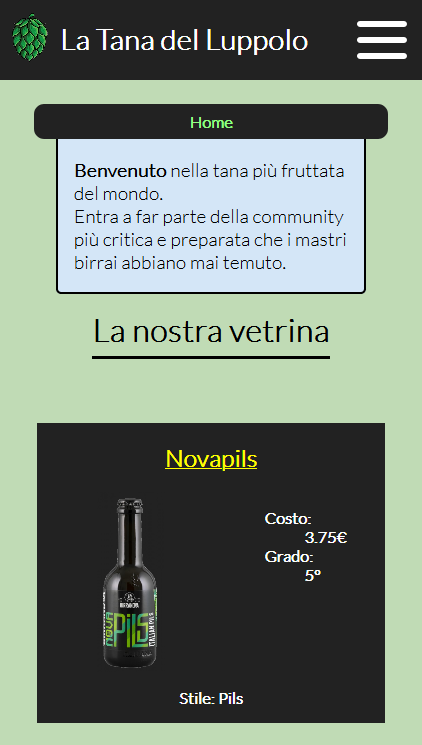
\includegraphics[width=6cm]{utility/home_mobile.png}
	\caption{Il layout mobile della homepage}
\end{figure}

Infine è stato predisposto un foglio di stile per la stampa dalla quale sono stati nascosti alcuni elementi giudicati superflui (ad esempio la barra di navigazione o i pulsanti Torna Su, ricerca e account) o modificati per migliorarne la presentazione (come la breadcrumb, le recensioni o la grandezza delle immagini principali).

\begin{figure}[H]
	\centering
	\caption{Il layout di stampa della pagina Prodotti}
	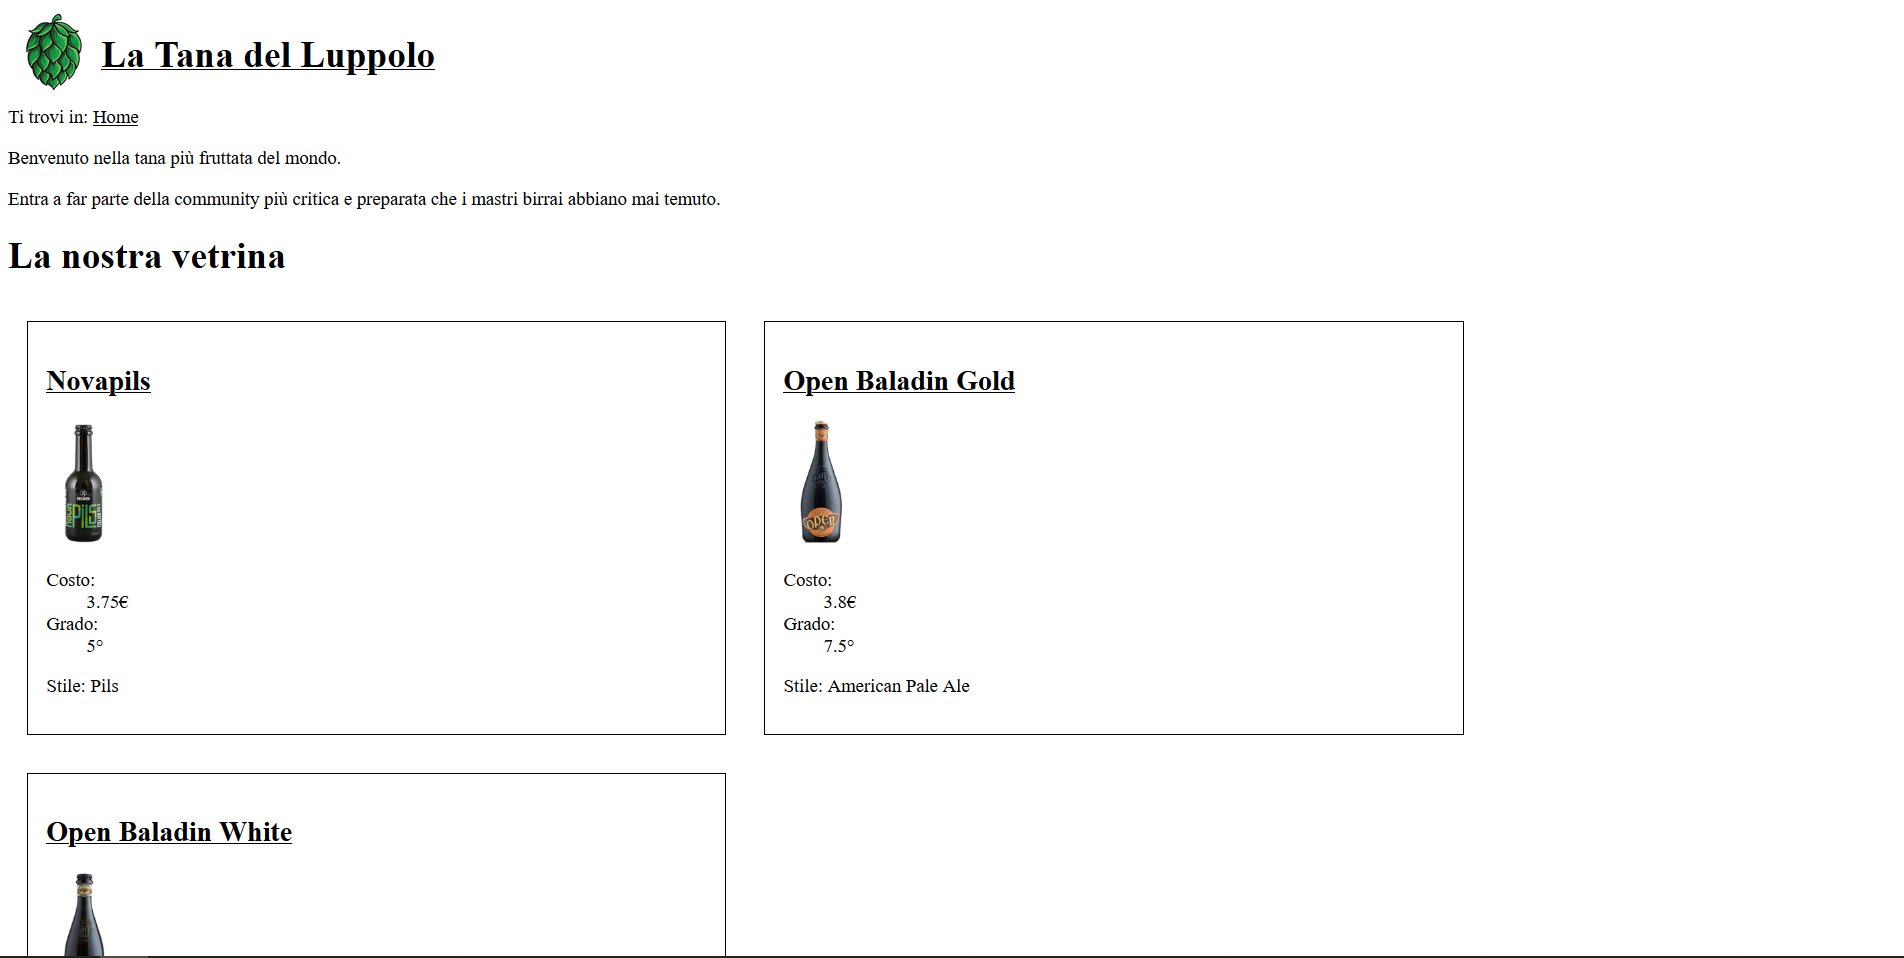
\includegraphics[width=16cm]{utility/prodotti_printcss.png}
\end{figure}

I colori dominanti del sito sono il grigio scuro e un verde pistacchio per header, sfondi ed altri elementi di presentazione mentre vengono utilizzati il nero, il verde ed il giallo per testi e link.\\

% palette colori
Sfondi ed elementi
\definecolor{hdgray}{RGB}{34, 34, 34}
\definecolor{pistacho}{RGB}{192, 219, 181}
\definecolor{puffo}{RGB}{212, 230, 247}
\crule[hdgray]{1cm}{1cm} \crule[pistacho]{1cm}{1cm} \crule[puffo]{1cm}{1cm} 


Testi e link
\definecolor{bcgreen}{RGB}{167, 255, 131}
\definecolor{hdgreen}{RGB}{216, 251, 216}
\crule{1cm}{1cm} \crule[yellow]{1cm}{1cm} \crule[bcgreen]{1cm}{1cm} \crule[hdgreen]{1cm}{1cm}
\\

La palette è stata scelta in modo da garantire una corretta visualizzazione anche da persone affette da diversi tipi di cecità o sensibilità del contrasto ed il contenuto del sito rimane correttamente visualizzabile anche senza il caricamento dello stile CSS.

\begin{figure}[H]
	\centering
	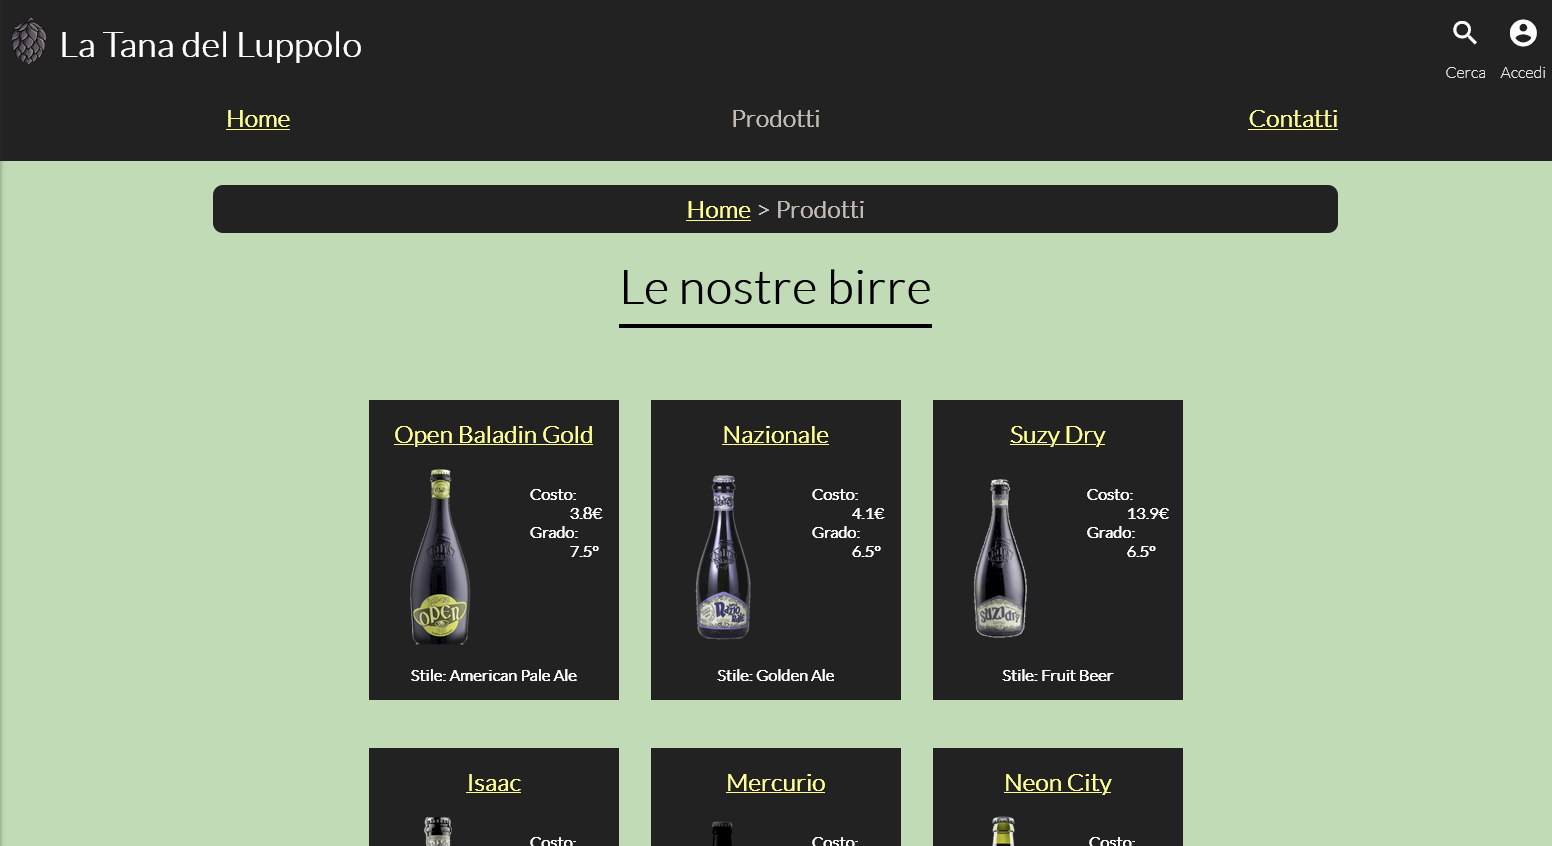
\includegraphics[width=16cm]{utility/prodotti_deuteranopia.png}
	\caption{Vista della pagina Prodotti da persone affette da deuteranopia (cecità al verde)}
\end{figure}


\subsection{Javascript}
\subsection{PHP}
Nel nostro sito, ogni pagina ha un suo file PHP, inoltre abbiamo creato due classi con metodi statici, così da non dover istanziare oggetti per richiamarne le funzioni:
\begin{itemize}
\item \textbf{htmlMaker.php:}
\item \textbf{dbConnection.php:}
\end{itemize}